\documentclass[12pt]{article}

\usepackage[table]{xcolor} % Para colores en tablas
\usepackage{booktabs}      % Para líneas profesionales
\usepackage{siunitx}       % Para unidades y alineación decimal
\usepackage{multirow}

% Codificación y fuentes
\usepackage[utf8]{inputenc}  % Ya no es necesario en distribuciones recientes (puedes usar sólo T1)
\usepackage[T1]{fontenc}      % Usar con \usepackage{lmodern} para mejor calidad
\usepackage{lmodern}          % Fuentes vectoriales modernas

% Idioma y tipografía
\usepackage[spanish]{babel}
\usepackage{microtype}        % Mejora el espaciado entre caracteres

% Matemáticas
\usepackage{amsmath}          % Entornos matemáticos
\usepackage{amssymb}         % Símbolos matemáticos
\usepackage{amsthm}          % Teoremas y pruebas
\usepackage{mathtools}       % Mejoras sobre amsmath (recomendado)

% Figuras y gráficos
\usepackage{graphicx}         % Inclusión de imágenes [scale, width, height]
\usepackage{subcaption}      % Sustituye a subfigure (para subfiguras)
\captionsetup{justification=centering} % Configuración de caption
\usepackage{graphicx} %insertar imagenes
\usepackage{float} %posicion exacta de figuras y tablas
% Paquetes necesario para trabajar con sub figuras
\usepackage{caption}

% Símbolos científicos
\usepackage{siunitx}         % Mejor que gensymb (para unidades, grados, etc.)
\sisetup{
    output-decimal-marker={,}, % coma decimal
    group-separator={.}        % punto para miles
}
% Referencias y citas
\usepackage[style=apa]{biblatex} % Moderno sistema de bibliografía
\addbibresource{bibliografia.bib} % Archivo .bib
\usepackage{hyperref}        % Links interactivos (debe ir al final)
\usepackage{cleveref}        % Referencias inteligentes

% Formato y diseño
\usepackage{parskip}         % Espaciado entre párrafos
\usepackage{fancyhdr}        % Encabezados personalizados
\usepackage[a4paper, margin=2.5cm]{geometry} % Márgenes
\usepackage{enumitem}        % Control avanzado de listas
\usepackage{booktabs} 

\title{Análisis de Elementos de Máquinas}
\author{Diego Müller, Valentina Larré, Felipe Sepúlveda}
\date{17 de julio de 2025}


\newcommand{\docent}{Ignacio Ríos}
\newcommand{\thetitle}{Diseño y cálculo del eje de un reductor de velocidad}
\newcommand{\theauthor}{Diego Müller, Valentina Larré, Felipe Sepúlveda}
\newcommand{\thedate}{17 de julio de 2025}
\newcommand{\thedocent}{\docent}

% Encabezados
\pagestyle{fancy}
\fancyhf{}
%\rhead{\theauthor}
\lhead{\thetitle}
\cfoot{\thepage}

\begin{document}

%%%%%%%%%%%%%%%%%%%%%%%%%%%%%%%%%%%%%%%%%%%%%%%%%%%%%%%%%%%%%%%%%%%%%%%%%%%%%%%%%%%%%%%%%

\begin{titlepage}
	\centering
    \vspace*{1cm}
    
\includegraphics[scale=0.7]{images/logoufro.png}\\[1cm]
    
    \textsc{\LARGE Universidad de La Frontera}\\[0.5cm]
	\textsc{\Large Departamento de Ingeniería Mecánica}\\[0.5cm]
	\textsc{\large Asignatura: Elementos de Máquinas}\\[0.8cm]
	
	\rule{\linewidth}{0.5mm} \\[0.4cm]
	{\huge \bfseries \thetitle}\\
	\rule{\linewidth}{0.3mm} \\[1.5cm]
	
	\textbf{Integrantes:}\\
	\theauthor\\[1cm]
    
    \textbf{Profesor:}\\
    \thedocent\\[1cm]

	\textbf{Fecha de entrega:} \\
	\thedate\\[2cm]
	
	\vfill
\end{titlepage}

%%%%%%%%%%%%%%%%%%%%%%%%%%%%%%%%%%%%%%%%%%%%%%%%%%%%%%%%%%%%%%%%%%%%%%%%%%%%%%%%%%%%%%%%%

\tableofcontents
\newpage

%%%%%%%%%%%%%%%%%%%%%%%%%%%%%%%%%%%%%%%%%%%%%%%%%%%%%%%%%%%%%%%%%%%%%%%%%%%%%%%%%%%%%%%%%

\section{Introducción}

Una empresa adquirió 30 cajas reductoras de velocidad destinadas al funcionamiento de sierras en una planta manufacturera. Cada unidad contaba con ejes que presentaban concentradores de esfuerzo, como zonas de chavetas y cambios de sección para el montaje de componentes, además de las áreas de contacto con rodamientos. La potencia era transmitida desde un motor eléctrico al eje de salida mediante engranajes rectos. Según lo indicado por el fabricante, estos reductores estaban diseñados para operar de forma continua durante un período de cinco años. Sin embargo, la unidad de mantenimiento reportó una vida útil significativamente menor.

Desde las áreas de operaciones e ingeniería se consideró que las fallas podrían deberse a un diseño inadecuado, mientras que el fabricante argumentó que estas se originaron por trabajar a potencias superiores a las especificadas, lo que habría generado sobrecargas en los componentes. Ante esta discrepancia, el superintendente de la planta asignó a un equipo de ingenieros la tarea de elaborar un informe de cálculo que permitiera evaluar técnicamente las causas de falla y, en caso de ser necesario, respaldar una posible reclamación al fabricante.

\subsection{Objetivos}
\begin{itemize}
    \item Determinar la vida útil de los ejes bajo las condiciones reales de operación y, si fuese necesario, rediseñarlos para cumplir con la vida útil especificada.
    \item Desarrollar una memoria de cálculo, considerando criterios de falla estáticos y por fatiga, junto con diagramas y ecuaciones analíticas.
    \item Modelar los componentes principales en software CAD y generar planos de fabricación con toda la información necesaria para su producción y montaje.
    \item Validar el diseño mediante simulaciones estructurales en software CAE, comparando los resultados con los cálculos teóricos.

\end{itemize}

\newpage
%%%%%%%%%%%%%%%%%%%%%%%%%%%%%%%%%%%%%%%%%%%%%%%%%%%%%%%%%%%%%%%%%%%%%%%%%%%%%%%%%%%%%%%%

\section{Caja reductora y condiciones del sistema}

Para el análisis de los ejes de la caja reductora de velocidad, se consideraron las siguientes condiciones operativas y parámetros de diseño:

\subsection{Parámetros de operación}
\begin{itemize}[leftmargin=*,nosep]
    \item \textbf{Potencia de entrada}: \SI{25}{hp}
    \item \textbf{Velocidad de entrada}: \SI{1750}{rpm}
    \item \textbf{Velocidad de salida}: \SI{500}{rpm}
    \item \textbf{Relación de transmisión}: 3{},5:1
\end{itemize}


\subsection{Tabla resumen de propiedades}
\begin{table}[h]
    \centering
    \caption{Resumen de parámetros de diseño y propiedades del material}
    \begin{tabular}{ll}
        \hline
        \textbf{Parámetro} & \textbf{Valor} \\
        \hline
        \multicolumn{2}{l}{\textbf{Datos operativos}} \\
        Potencia de entrada & \SI{25}{hp}  \\
        Velocidad de entrada & \SI{1750}{rpm} \\
        Velocidad de salida & \SI{500}{rpm} \\
        Relación de transmisión & 3,5:1 \\
        \hline
        \multicolumn{2}{l}{\textbf{Geometría de engranajes}} \\
        Diámetro engranaje (nombrar) & \SI{3,75}{in} \\
        \hline
        \multicolumn{2}{l}{\textbf{Propiedades del material (SAE 1144)}} \\
        Esfuerzo último ($S_u$) & 118000\ \text{psi} \\
        Límite de fluencia ($S_y$) & 83000\ \text{psi} \\
        Módulo de elasticidad ($E$) & \SI{29,700}{ksi} \\
        \hline
    \end{tabular}
    \label{tab:resumen1}
\end{table}


\subsection{Diseño}

En la Figura~\ref{fig:subfigs} se presenta el diseño del sistema reductor de velocidad, donde se detallan sus vistas principales.

\begin{figure}[H]
    \centering
    \begin{subfigure}[b]{0.46\textwidth}
        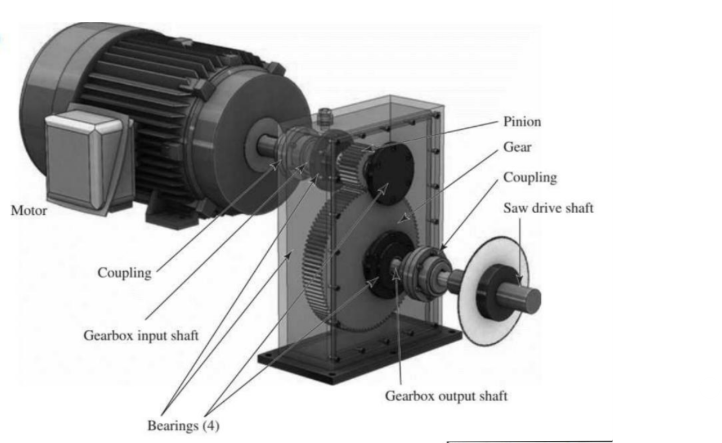
\includegraphics[width=\textwidth]{images/caja reductora.png}
        \caption{Vista isométrica.}
        \label{fig:sub1}
    \end{subfigure}
    \hfill % Espacio horizontal
    \begin{subfigure}[b]{0.46\textwidth}
        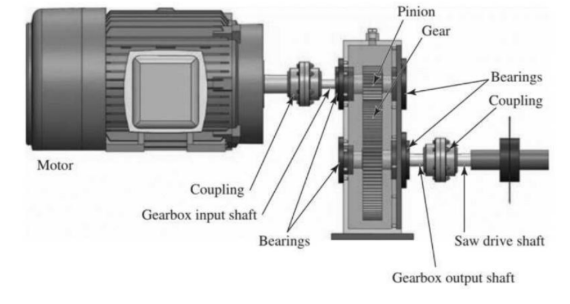
\includegraphics[width=\textwidth]{images/cajareductora_frente.png}
        \caption{Vista lateral.}
        \label{fig:sub2}
    \end{subfigure}
    \caption{Sistema caja reductora.}
    \label{fig:subfigs}
\end{figure}
\subsubsection{Descripción de componentes}
El sistema reductor de velocidad está compuesto por los siguientes elementos:

\begin{itemize}
    \item \textbf{Motor eléctrico}: Dispositivo que entrega la potencia mecánica al sistema. En este caso, proporciona una potencia nominal de 25 hp a una velocidad constante de 1750 rpm.
    \item \textbf{Acoplamiento (Coupling):}: Elemento flexible utilizado para conectar el eje del motor con el eje de entrada de la caja reductora. Su función es transmitir el torque minimizando desalineaciones y vibraciones.
    \item \textbf{Eje de entrada de la caja reductora (Gearbox input shaft)}: Eje que recibe el movimiento rotacional del motor y lo transmite al sistema de engranajes internos de la caja.
    \item \textbf{Conjunto de rodamientos (Bearings)}: Soportes mecánicos que permiten la rotación del eje con baja fricción y mantienen su alineación. En este sistema se identifican cuatro rodamientos.
     \item \textbf{Piñón (Pinion)}:Engranaje de menor diámetro montado en el eje de entrada. Se acopla al engranaje mayor para reducir la velocidad y aumentar el torque.
     \item \textbf{Engranaje (Gear)}:Engranaje de mayor tamaño conectado al piñón. Está montado sobre el eje de salida y forma parte del tren reductor. Su relación de transmisión con el piñón define la reducción de velocidad.
     \item \textbf{Eje de salida de la caja reductora (Gearbox output shaft)}:Eje que entrega el movimiento rotacional reducido al sistema de corte. Su velocidad es menor pero el torque es mayor en comparación con el eje de entrada.
     \item \textbf{Acoplamiento secundario (Coupling)}: Elemento adicional que conecta el eje de salida con el eje de la sierra, permitiendo una transmisión eficiente y flexible.
     \item \textbf{Eje de la sierra (Saw drive shaft)}:Eje final del sistema, donde se monta la sierra de corte. Recibe el torque amplificado y lo transforma en movimiento útil para el proceso de corte.
    

\subsubsection{Planos de los ejes}

La \textbf{geometría completa de los ejes}, tal como se ilustra en la Figura~\ref{fig:subfigs2}, presenta una complejidad que dificulta un análisis teórico directo. Para facilitar este análisis y concentrarnos en las áreas de mayor interés, se ha procedido con una \textbf{simplificación de la geometría}. La simplificación se enfoca en mantener solo las características dimensionales críticas y que, por su magnitud son las principales responsables de generar concentraciones de esfuerzo. 

\begin{figure}[H]
    \centering
    \begin{subfigure}[b]{0.46\textwidth}
        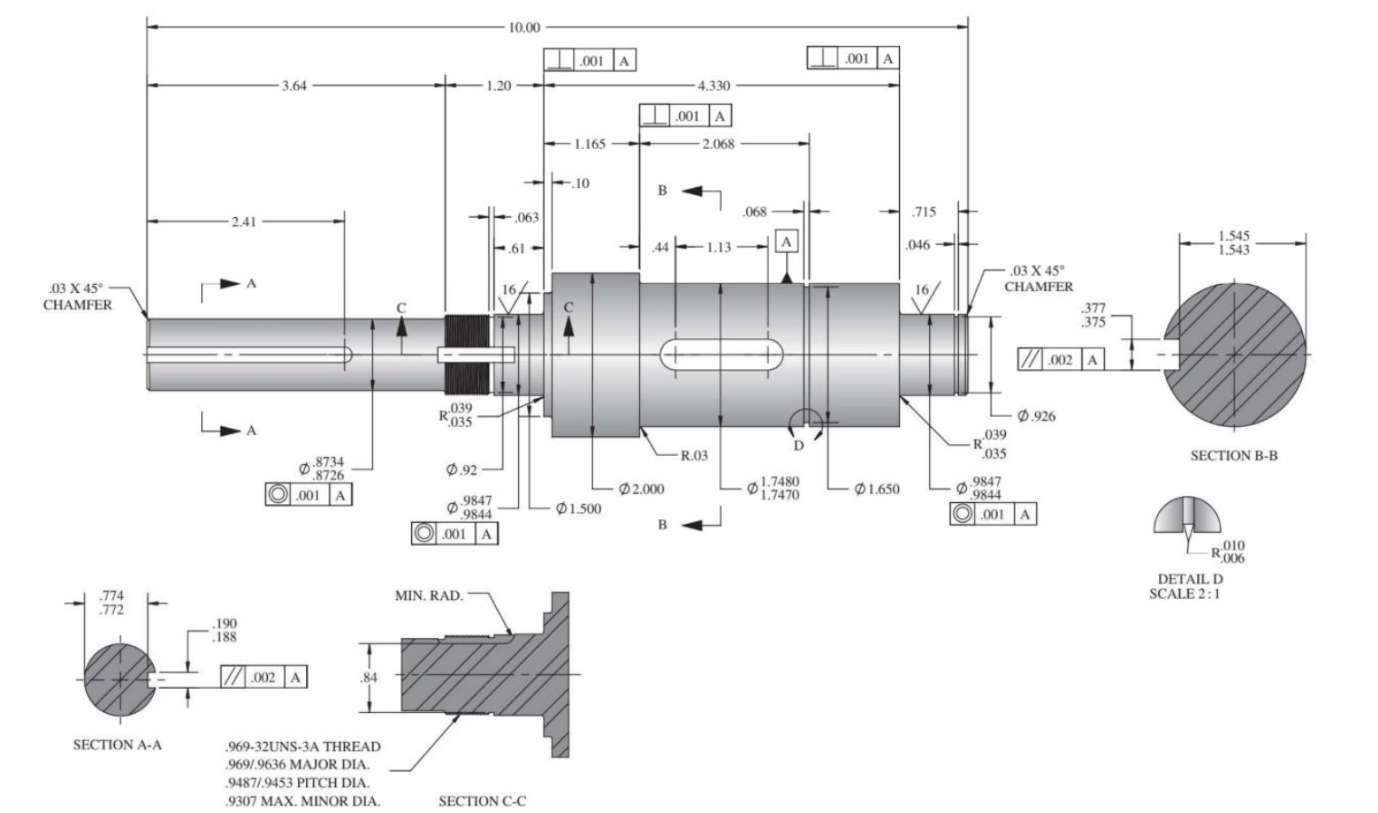
\includegraphics[width=\textwidth]{images/ejeentradadet.png}
        \caption{Plano eje de entrada detallado.}
        \label{fig:sub21}
    \end{subfigure}
    \hfill % Espacio horizontal
    \begin{subfigure}[b]{0.46\textwidth}
        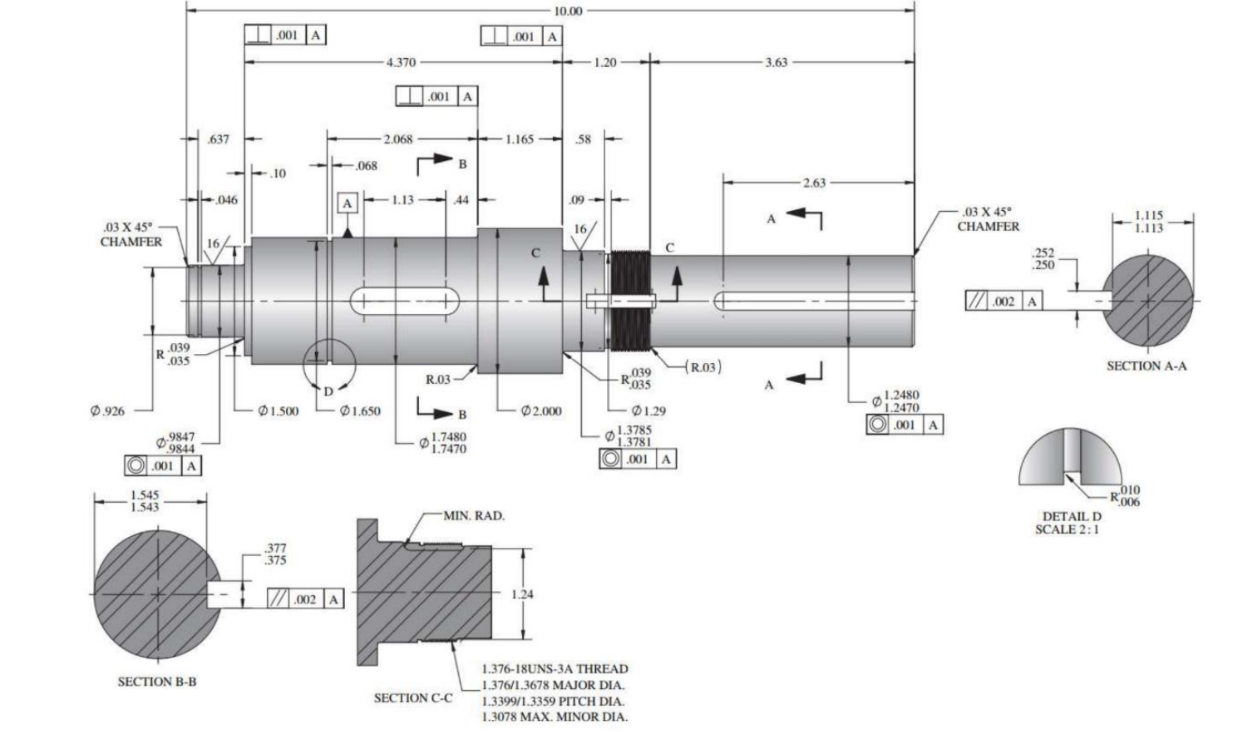
\includegraphics[width=\textwidth]{images/ejesalidadet.png}
        \caption{Plano eje de salida detallado.}
        \label{fig:sub22}
    \end{subfigure}
    \caption{Planos detallados de los ejes.}
    \label{fig:subfigs2}
\end{figure}
\end{itemize}
\subsubsection{Engranajes}
\textbf{Ángulo de presión:}

El ángulo de presión (\( \phi = 20^\circ \)) es el valor estándar más comúnmente utilizado en engranajes rectos industriales, ya que representa un buen equilibrio entre resistencia a la carga, eficiencia de transmisión y facilidad de fabricación. Un ángulo menor reduciría la fuerza radial, pero comprometería la robustez del engranaje. Por ello, para el análisis se mantiene el valor de \(20^\circ\), recomendado también por el libro de Shigley como típico para engranajes involutos.

\begin{figure}[H]
    \centering
    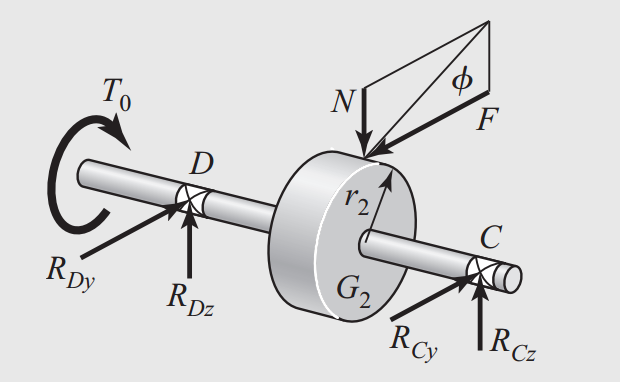
\includegraphics[width=0.5\textwidth]{images/engranaje.png}
\caption{Representación ángulo de presión $\phi$.}
    \label{fig:engranajephi}
\end{figure}



\subsection{Cálculo del torque}

El torque transmitido se calcula mediante \parencite{budynas2012diseño}:
\begin{equation}
\label{eq:torque}
T = \frac{P \times C}{n}
\end{equation}
donde:
\begin{itemize}[leftmargin=2cm,nosep]
    \item[$T$:] Torque transmitido (\SI{}{lb\cdot in})
    \item[$P$:] Potencia del motor (\SI{}{hp})
    \item[$n$:] Velocidad de rotación (\SI{}{rpm})
    \item[$C$:] Factor de conversión = 63025 [\text{lb·in·rpm/hp}]
\end{itemize}

\begin{table}[h]
\centering
\caption{Resultados de torque para diferentes velocidades}
\begin{tabular}{lcc}
\hline
Eje & Velocidad (rpm) & Torque (lb·in) \\
\hline
Entrada & 500 & 3151,25 \\
Salida & 1750 & 900,36 \\
\hline
\end{tabular}
\end{table}



\subsection{Eje de entrada}

\begin{figure}[H]
    \centering
    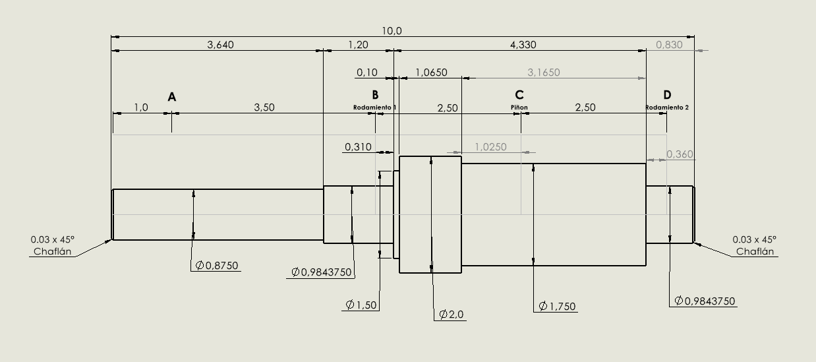
\includegraphics[width=0.85\textwidth]{images/ejeentradasimple.png}
    \caption{Plano eje de entrada simple.}
    \label{fig:eje_entrada}
\end{figure}


\subsubsection{Velocidad en la línea de paso del engranaje}
agregar que es la linea de paso

\begin{equation}
V_{línea} = \frac{\pi \cdot d \ \cdot n}{12}=\frac{\pi \cdot 3.75 \cdot 1750}{12} \approx 1718.06\ \text{ft/min}
\end{equation}
\begin{itemize}[leftmargin=2cm,nosep]
    \item[$V_{línea}$:] Velocidad en la línea de paso \SI{}{ft/min}
    \item[$d$:] Diámetro del engranaje (\SI{}{in})
    \item[$n$:] Velocidad de rotación (\SI{}{rpm})
    
\end{itemize}

\subsubsection{Fuerza tangencial transmitida por el engranaje}
Se usa la siguiente relación, derivada del equilibrio de potencia:
\begin{equation}
W_t = \frac{33000 \cdot P}{V_{línea}} = \frac{33000 \cdot 25}{1718.06} \approx\ \SI{480.19}{lb}
\end{equation}

\begin{itemize}[leftmargin=2cm,nosep]
    \item[$V_{línea}$:] Velocidad de linea de paso (\SI{}{ft/min})
    \item[$P$:]Potencia (\SI{}{hp})   
\end{itemize}

\subsubsection{Fuerza radial}
La fuerza radial depende del ángulo de presión del engranaje:
\begin{equation}
W_r = W_t \cdot \tan(\phi)= 480.19 \cdot \tan(20^\circ) \approx 174.78\ \text{lb}
\end{equation}
\begin{itemize}[leftmargin=2cm,nosep]
    \item[$\phi$:] Ángulo de presión (20° típico en engranajes rectos)
\end{itemize}

\subsubsection{Fuerza total aplicada sobre el engranaje}
\begin{equation}
W = \sqrt{W_t^2 + W_r^2} = \sqrt{(480.19)^2 + (174.78)^2} \approx 511.01\ \text{lb}
\end{equation}

%%%%%%%%%%%%%%%%%%%%%%%%%%%%%%%%%%%%%%%%%%%%%%%%%%%%%%%%%%%%%%%%
\subsection{Eje de salida}

\begin{figure}[H]
    \centering
    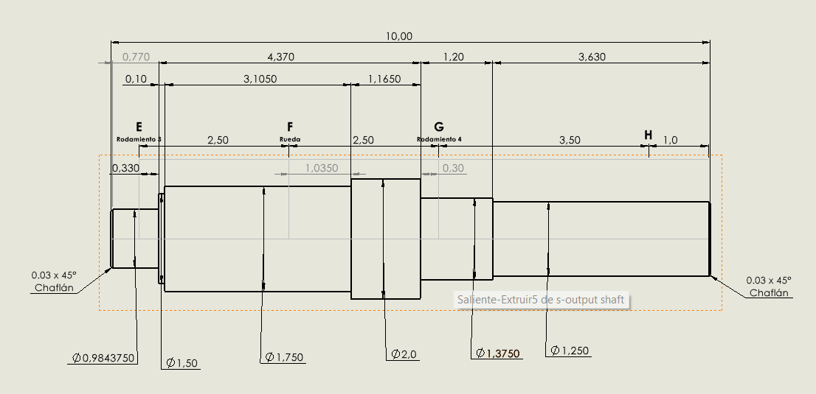
\includegraphics[width=0.85\textwidth]{images/ejesalidasimple.png}
    \caption{Plano eje de salida simple.}
    \label{fig:eje_salida}
\end{figure}

Para el análisis del eje de salida, se consideran las cargas aplicadas por el engranaje impulsado, calculadas a partir del torque transmitido. Los cálculos se realizan en base a la misma metodología aplicada al eje de entrada.

\vspace{0.2cm}

\noindent


\subsubsection{Velocidad en la línea de paso:}
\begin{equation}
V = \frac{\pi \cdot d \cdot n}{12} = \frac{\pi \cdot 13.125 \cdot 500}{12} \approx 1718.06\ \text{ft/min}
\end{equation}
\begin{itemize}[leftmargin=2cm,nosep]
    \item[$d$:] Diámetro del engranaje (13.125 in)
    \item[$n$:] Velocidad angular (500 rpm)
\end{itemize}

\vspace{0.2cm}

\noindent
\subsubsection{Fuerza tangencial:}
\begin{equation}
W_t = \frac{33,000 \cdot H}{V} = \frac{33,000 \cdot 25}{1718.06} \approx 480.19\ \text{lb}
\end{equation}
\begin{itemize}[leftmargin=2cm,nosep]
    \item[$H$:] Potencia del motor (25 hp)
    \item[$V$:] Velocidad en la línea de paso (ft/min)
\end{itemize}

\vspace{0.2cm}

\noindent
\subsubsection{Fuerza radial:}
\begin{equation}
W_r = W_t \cdot \tan(\phi) = 480.19 \cdot \tan(20^\circ) \approx 174.78\ \text{lb}
\end{equation}
\begin{itemize}[leftmargin=2cm,nosep]
    \item[$\phi$:] Ángulo de presión (20° típico en engranajes rectos)
\end{itemize}

\vspace{0.2cm}

\noindent
\subsubsection{Fuerza total aplicada sobre el engranaje:}
\begin{equation}
W = \sqrt{W_t^2 + W_r^2} = \sqrt{(480.19)^2 + (174.78)^2} \approx 511.01\ \text{lb}
\end{equation}

\vspace{0.3cm}

\noindent

\subsection{Resumen de parámetros en ejes}
\begin{table}[H]
\centering
\caption{Resumen de fuerzas y parámetros en los ejes de entrada y salida}
\label{tab:resumen2}
\begin{tabular}{lcc}
\toprule
\textbf{Parámetro} & \textbf{Eje de entrada} & \textbf{Eje de salida} \\
\midrule
Velocidad (rpm) & 1750 & 500 \\
Torque (lb$\cdot$in) & 900,36 & 3151,25
 \\
Diámetro engranaje (in) & 3,75 & 13,125 \\
Velocidad línea de paso (ft/min) & 1718,06 & 1718,06 \\
Fuerza tangencial, $W_t$ (lb) & 480,19 & 480,19 \\
Fuerza radial, $W_r$ (lb) & 174,78 & 174,78 \\
Fuerza resultante, $W$ (lb) & 511,01 & 511,01 \\
\bottomrule
\end{tabular}
\end{table}


%%%%%%%%%%%%%%%%%%%%%%%%%%%%%%%%%%%%%%%%%%%%%%%%%%%%%%%%%%%%%%%%%%%%%
\section{Análisis teórico}
Según lo estudiado y enfoque de diseño, un eje debe ser dimensionado considerando \parencite[]{budynas2012diseño}:
 \begin{itemize}
     \item Cargas aplicadas : Fuerzas tangenciales, radiales y axiales transmitidas por engranajes o poleas.
     \item Esfuerzos (torsión, flexión, cortante y axial).
     \item Concentradores de esfuerzo (cambios de sección, chaveteros, radios, etc.).
     \item Fatiga y confiabilidad (para cargas cíclicas).
     \item Selección de material y factor de seguridad.
 \end{itemize}

\subsection{Cargas y momentos}
Se inicia con el estudio de las cargas y reacciones en el eje de entrada, considerando las reacciones en los cojinetes y transmisión de potencia.

\begin{figure}[H]
    \centering
    \begin{subfigure}[b]{0.85\textwidth}
        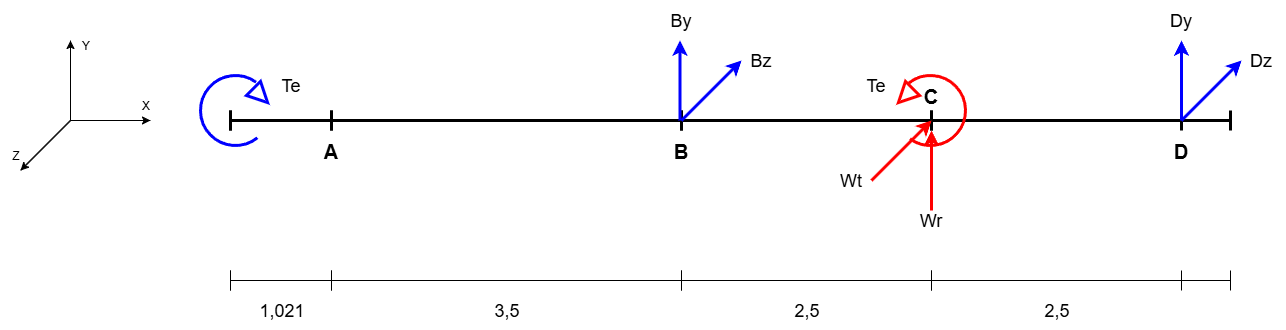
\includegraphics[width=\textwidth]{imagenes dcl/entradcl.drawio.png}
        \caption{DCL eje de entrada.}
        \label{fig:entrada22}
    \end{subfigure}
    \hfill % Espacio horizontal
    \begin{subfigure}[b]{0.85\textwidth}
        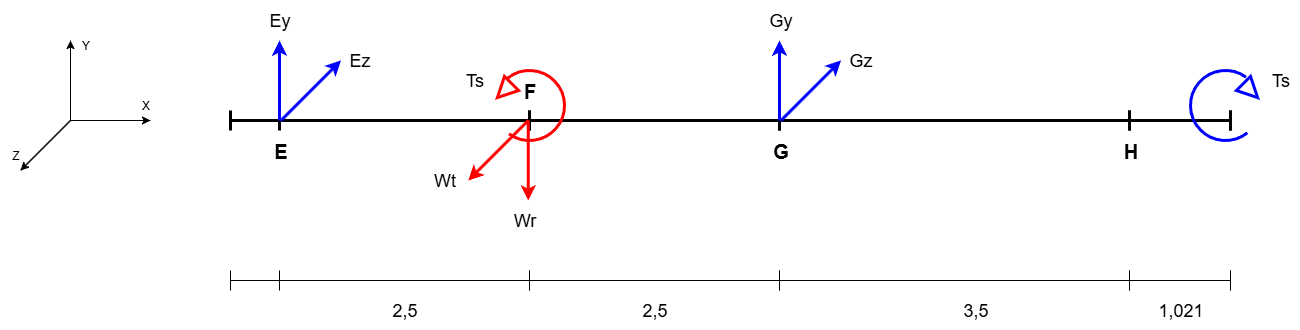
\includegraphics[width=\textwidth]{imagenes dcl/ejesalida.png}
        \caption{DCL eje de salida.}
        \label{fig:salida2}
    \end{subfigure}
    \caption{DCL para ambos ejes.}
    \label{fig:dcl_ejes}
\end{figure}


\subsubsection{Cargas aplicadas}
En el sistema simétrico, las fuerzas se dividen equitativamente entre los apoyos:

\begin{table}[H]
\centering
\caption{Cargas aplicadas sobre el eje}
\label{tab:cargas}
\begin{tabular}{lc}
\toprule
\textbf{Carga} & \textbf{Valor (lb o lb·in)} \\
\midrule
Momento torsor ($T$) & 900.35 \\
Fuerza radial ($W_r$) & 174.78 \\
Fuerza tangencial ($W_t$) & 480.19 \\
\bottomrule
\end{tabular}
\end{table}

\textbf{Reacciones en los cojinetes: }\\
Dada la equidistancia de las fuerzas aplicadas, cada reacción en los soportes de los ejes se distribuye por igual. Por lo tanto, cada cojinete soporta la mitad del valor total de la fuerza, tal como se ilustra en el diagrama de cuerpo libre mostrado en la Figura~\ref{fig:dclreay}. Esta misma condición de distribución equitativa de las reacciones aplica para el plano X-Z. Los valores específicos de las reacciones calculadas para cada cojinete se presentan en el cuadro 5.

\begin{figure}[H]
    \centering
    \begin{subfigure}[b]{0.85\textwidth}
        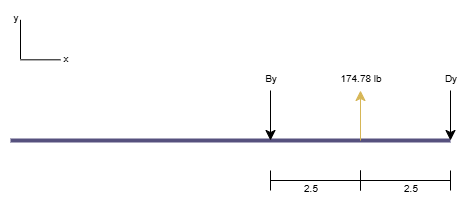
\includegraphics[width=\textwidth]{imagenes dcl/diareaeje.png}
        \caption{DCL reacciones eje de entrada.}
        \label{fig:entrada3}
    \end{subfigure}
    \hfill % Espacio horizontal
    \begin{subfigure}[b]{0.85\textwidth}
        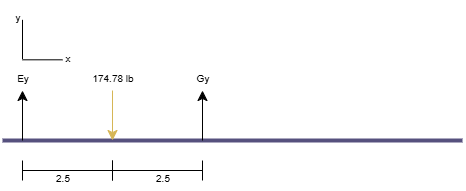
\includegraphics[width=\textwidth]{imagenes dcl/salidarea w.png}
        \caption{DCL reacciones eje de salida.}
        \label{fig:salida33}
    \end{subfigure}
    \caption{DCL para ambos ejes.}
    \label{fig:dclreay}
\end{figure}


\begin{table}[H]
\centering
\caption{Reacciones en los rodamientos (valores en lb)}
\label{tab:reacciones}
\begin{tabular}{lcccc}
\toprule
\multirow{2}{*}{\textbf{Componente}} & \multicolumn{4}{c}{\textbf{Rodamiento}} \\
\cmidrule{2-5}
 & \textbf{B} & \textbf{D} & \textbf{E} & \textbf{G} \\
\midrule
Vertical ($R_y$) & 87.39 & 87.39 & 87.39 & 87.39 \\
Horizontal ($R_z$) & 240.10 & 240.10 & 240.10 & 240.10 \\
\bottomrule
\end{tabular}
\end{table}

Donde:
\begin{itemize}[leftmargin=2cm, nosep]
\item $R_y = \frac{W_r \cdot \SI{2.5}{in}}{\SI{5}{in}} = \frac{174.78 \cdot 5 in }{2.5 in} =  87.39\ \text{lb}$
\item $R_z = \frac{W_t \cdot \SI{2.5}{in}}{\SI{5}{in}} = \frac{480.19 \cdot 5 in }{2.5 in} =  240,10 \ \text{lb}$
\end{itemize}

%%%%%% esperar datos actualizados 
\subsection{Análisis en el eje de entrada}
Los momentos para los puntos de interés del eje de entrada se ven en el siguiente cuadro.

\begin{table}[h]
\centering
\caption{Momentos flectores en el eje - Detallado}
\label{tab:momentos_detallados}
\rowcolors{2}{gray!10}{white} % Fondo alternado para mejor legibilidad
\begin{tabular}{l S[table-format=1.6] S[table-format=-3.6] S[table-format=-3.6] S[table-format=3.6]}
\toprule
\textbf{Punto} & \textbf{X [\si{in}]} & \textbf{My [\si{lb\cdot in}]} & \textbf{Mz [\si{lb\cdot in}]} & \textbf{M total [\si{lb\cdot in}]} \\
\midrule
A/ranura1       & 1.02 &     0.0 &     0.0 &     0.0 \\
ranura1final    & 2.41 &     0.0 &     0.0 &     0.0 \\ \rowcolor{green!30}
Filete1         & 3.63 &     0.0 &     0.0 &     0.0 \\
ranura2inicio   & 3.64 &     0.0 &     0.0 &     0.0 \\
ranura2final    & 4.14 &     0.0 &     0.0 &     0.0 \\ \rowcolor{green!30}
B               & 4.52 &     0.0 &     0.0 &     0.0 \\
Filete2         & 4.83 &    27.09 &    74.43 &    79.21 \\
Filete3         & 4.93 &    35.82 &    98.44 &   104.76 \\ \rowcolor{blue!10}
I               & 5.41 &    77.99 &   214.29 &   228.04 \\
Filete4         & 5.99 &   128.90 &   354.15 &   376.88 \\ \rowcolor{green!30}
ranura3inicio   & 6.45 &   169.09 &   464.59 &   494.41 \\
C               & 7.02 &   218.4 &   600.25 &   638.77 \\
ranura3final    & 7.59 &   169.09 &   464.59 &   494.42 \\ \rowcolor{blue!10}
anillo1         & 8.06 &   127.33 &   349.84 &   372.29 \\
Filete5         & 9.16 &    31.46 &    86.46 &    92 \\ \rowcolor{green!30}
D               & 9.52 &     0.0 &     0.0 &     0.0 \\
anillo2         & 9.88 &     0.0 &     0.0 &     0.0 \\
\bottomrule
\end{tabular}
\end{table}




\subsubsection{Cargas aplicadas}
\begin{table}[H]
\centering
\caption{Cargas aplicadas sobre el eje de salida}
\label{tab:cargas_salida}
\begin{tabular}{lc}
\toprule
\textbf{Carga} & \textbf{Valor} \\
\midrule
Momento torsor ($T$) & \SI{3151.25}{lb\cdot in} \\
Fuerza radial ($W_r$) & \SI{174.78}{lb} \\
Fuerza tangencial ($W_t$) & \SI{480.19}{lb} \\
\bottomrule
\end{tabular}
\end{table}


\begin{itemize}[leftmargin=2cm, nosep]
\item Cálculo de reacciones verticales: $R_y = \frac{W_r}{2} = \frac{\SI{174.78}{lbf}}{2} = \SI{87.39}{lb}$
\item Cálculo de reacciones horizontales: $R_z = \frac{W_t}{2} = \frac{\SI{480.19}{lbf}}{2} = \SI{240.10}{lb}$
\end{itemize}


%%%%%%%%%%%%%%%%%%%%%%%%%%%%%%%%%%%%%%%%%%%%%%%%%%%%%%%%%%%%%%%%
\section{Resultados}
Presenta los resultados obtenidos a partir del análisis. Puedes usar tablas, gráficos o figuras si es necesario.

\section{Conclusiones}
Redacta las conclusiones principales del informe, las lecciones aprendidas, posibles mejoras y recomendaciones.


\printbibliography

\end{document}